\chapter{Un cadre bayésien pour la détection de communautés sur graphes}
\label{chap:bayes_clusters_graphes}

\providecommand{\SW}{\textnormal{\textsc{Swendsen--Wang}}}
\providecommand{\ES}{\textnormal{\textsc{Edwards--Sokal}}}
\providecommand{\KBD}{\textnormal{\textsc{Kandel--Ben-Av--Domany}}}
\providecommand{\SB}{\textnormal{\textsc{Sankararaman--Baccelli}}}
\providecommand{\EA}{\textnormal{\textsc{Edwards--Anderson}}}
\providecommand{\Obs}{\mathcal O}
\providecommand{\Conf}{\mathcal S}
\providecommand{\Lab}{\mathsf S}
\providecommand{\Wspace}{\mathsf W}
\providecommand{\Sorties}{\mathcal A}
\providecommand{\Loi}{\mathcal L}
\providecommand{\RG}{\operatorname{RG}}
\providecommand{\ov}{\operatorname{ov}}
\providecommand{\sgn}{\operatorname{sgn}}
\providecommand{\Id}{\operatorname{Id}}
\providecommand{\supp}{\operatorname{supp}}
\providecommand{\ind}[1]{\mathds{1}_{\{#1\}}}
\providecommand{\eps}{\varepsilon}

\usetikzlibrary{fit,backgrounds,shapes.geometric,patterns,decorations.pathreplacing}
\tikzset{
  chapbox/.style={draw,rounded corners,very thick,align=center,fill=gray!8,inner sep=5pt,minimum height=1.05cm},
  chapboxdark/.style={draw,rounded corners,very thick,align=center,fill=gray!18,inner sep=5pt,minimum height=1.05cm},
  chaparr/.style={-{Latex[length=2.4mm]},very thick},
  chapdash/.style={-{Latex[length=2.4mm]},very thick,dashed},
  spin/.style={circle,draw,inner sep=0pt,minimum size=5mm,font=\scriptsize,fill=white},
  tinynode/.style={circle,draw,inner sep=0pt,minimum size=3.8mm,font=\tiny,fill=white},
  posedge/.style={line width=1pt},
  negedge/.style={line width=1pt,dashed},
  freeze/.style={line width=1.6pt},
  faint/.style={line width=.45pt,gray!55},
  triwhite/.style={draw,fill=gray!8,line width=.6pt},
  trigray/.style={draw,fill=gray!22,line width=.6pt}
}



Ce chapitre s'intéresse au cas où les données en entrée ont une structure de graphe. Le clustering sur les nœuds s'appelle alors dans ce domaine \emph{détection de communauté sur graphes} \cite{AvrachenkovDreveton2022}.

L'objectif de ce chapitre est triple : 
\begin{enumerate}
    \item Toute la première partie consiste à donner un cadre bayésien rigoureux au problème de {détection de communauté sur graphes} : \emph{a priori}, algorithmes, canal d'observation, postérieure, tirages au hasard (\emph{random guess} en anglais) et recouvrement partiel (\emph{weak/partial recovery} en anglais).
    \item La seconde partie introduit une famille de dynamiques de clusters généralisant \SW{}.
    \item La troisième partie applique le cadre bayésien au modèle de \SB{} et montre comment retrouver simplement dans ce cadre leurs résultats de \cite{SankararamanBaccelli2018}, et comment une dynamique triangulaire permet d'obtenir des bornes plus fines (cas particulier de la grille triangulaire).
\end{enumerate}

\begin{figure}[H]
\centering
\begin{tikzpicture}[node distance=1.1cm and 1.2cm]
  \node[chapboxdark,minimum width=4.1cm] (p1) {Cadre bayésien};
  \node[chapboxdark,minimum width=4.1cm,right=of p1] (p2) {Dynamiques de clusters};
  \node[chapboxdark,minimum width=4.1cm,right=of p2] (p3) {Applications};
  \draw[chaparr] (p1) -- (p2);
  \draw[chaparr] (p2) -- (p3);
  \node[chapbox,minimum width=3.3cm,below=.9cm of p1] (b1) {$\mu_0$, observation,\\postérieure $\mu_{x,w}$};
  \node[chapbox,minimum width=3.3cm,below=.9cm of p2] (b2) {transition $M_{x,w}$\\invariante};
  \node[chapbox,minimum width=3.3cm,below=.9cm of p3] (b3) {percolation\\et bornes};
  \draw[chaparr] (p1) -- (b1);
  \draw[chaparr] (p2) -- (b2);
  \draw[chaparr] (p3) -- (b3);
\end{tikzpicture}
\caption{Architecture du chapitre. }
\label{fig:chapII_architecture}
\end{figure}


\Contributions{Ce chapitre reprend et affine un premier travail préparatoire consacré aux dynamiques de clusters d'ordre supérieur pour la détection de communautés dans des graphes euclidiens \cite{BibiMonterey}. (Il fera l'objet d'une soumission à un journal.) }

\section{Cadre bayésien général}
\addcontentsline{toc}{section}{Sous-partie I --- Cadre bayésien général}
\label{sec:chapII_partie_bayes}

\section{Modèle probabiliste, postérieure et algorithmes}
\label{sec:chapII_modele_bayesien}

\subsection{L'espace produit probabilisé}

Pour chaque $n\geq1$, on fixe un ensemble de sommets
\[
    V_n=\{1,\ldots,n\},
\]
un ensemble d'arêtes potentielles
\[
    E_n\subseteq \binom{V_n}{2},
\]
et un ensemble de \emph{communautés} (désignant dans le domaine des graphes les clusters, aussi souvent appelés \emph{labels})
\[
    \Lab_K=\{1,\ldots,K\},\qquad K\geq2.
\]
L'espace des configurations est
\[
    \Conf_n=\left(\Lab_K\right)^{V_n}.
\]
Une configuration sera notée $\sigma=(\sigma_i)_{i\in V_n}$.

Les poids observés prennent leurs valeurs dans un espace mesurable $\Wspace$. Dans les applications principales, on prendra $\Wspace\subseteq\mathbb R\cup\{\pm\infty\}$ : un poids positif indique une tendance à avoir le même label, un poids négatif indique une tendance à avoir des labels différents. Mais le cadre bayésien ci-dessous n'impose pas cette interprétation dès le départ.

\begin{Definition}{Modèle bayésien de détection de communautés}{chapII_modele_bayesien}
Un modèle bayésien de détection de communautés est la donnée, pour chaque $n$, des objets suivants.
\begin{enumerate}
    \item Un espace mesurable de traits observables $\mathcal X_n$ et une variable
    \[
        X_n\in\mathcal X_n
    \]
    de loi $\nu_n$.
    \item Un a priori, éventuellement dépendant des traits,
    \[
        \mu_{0,n}(\mathrm d\sigma\mid x),\qquad \sigma\in\Conf_n.
    \]
    Lorsque l'a priori ne dépend pas de $x$, on écrit simplement $\mu_{0,n}$.
    \item Un canal d'observation
    \[
        Q_n(\mathrm dw\mid x,\sigma)
    \]
    de $\mathcal X_n\times\Conf_n$ vers $\Wspace^{E_n}$.
\end{enumerate}
La loi jointe de $(X_n,\Sigma_n,W_n)$ est
\begin{equation}
    \mathbb P_n(\mathrm dx,\mathrm d\sigma,\mathrm dw)
    =
    \nu_n(\mathrm dx)\,\mu_{0,n}(\mathrm d\sigma\mid x)\,Q_n(\mathrm dw\mid x,\sigma).
    \label{eq:chapII_loi_jointe_generale}
\end{equation}
L'observation disponible est
\[
    \Obs_n=(X_n,W_n).
\]
\end{Definition}

Dans les modèles à arêtes conditionnellement indépendantes, le canal se factorise sous la forme
\begin{equation}
    Q_n(\mathrm dw\mid x,
    \sigma)
    =
    \prod_{e=\{i,j\}\in E_n}Q_{e,n}(\mathrm dw_e\mid x_i,x_j,\sigma_i,\sigma_j).
    \label{eq:chapII_canal_produit}
\end{equation}
Cette forme inclut les modèles où
\[
    W_e=f_e(X_i,X_j,\Sigma_i,\Sigma_j,U_e),
\]
avec des variables auxiliaires indépendantes $(U_e)_{e\in E_n}$.

\paragraph{Postérieure.}
On suppose les espaces standard boréliens, ce qui est le cas dans les applications finies de ce chapitre. Il existe alors une loi conditionnelle régulière de $\Sigma_n$ sachant l'observation. On la note
\begin{equation}
    \mu_{n,x,w}(\mathrm d\sigma)
    =
    \mathbb P_n\left[\Sigma_n\in\mathrm d\sigma\mid X_n=x,W_n=w\right].
    \label{eq:chapII_posterieure_def}
\end{equation}
Lorsque $Q_n$ admet une densité $q_n(w\mid x,\sigma)$ par rapport à une mesure de référence, on obtient
\begin{equation}
    \mu_{n,x,w}(\sigma)
    =
    \frac{1}{Z_n(x,w)}\,
    \mu_{0,n}(\sigma\mid x)\,q_n(w\mid x,\sigma).
    \label{eq:chapII_posterieure_densite}
\end{equation}
La constante $Z_n(x,w)$ normalise la mesure.

\begin{figure}[H]
\centering
\begin{tikzpicture}[node distance=1cm and 1.25cm]
  \node[chapbox,minimum width=3.1cm] (prior) {a priori\\$\mu_{0,n}(\cdot\mid X)$};
  \node[chapbox,minimum width=3.1cm,right=of prior] (truth) {vérité cachée\\$\Sigma_n$};
  \node[chapbox,minimum width=3.1cm,right=of truth] (chan) {canal\\$Q_n$};
  \node[chapboxdark,minimum width=3.1cm,right=of chan] (obs) {observation\\$\Obs_n=(X,W)$};
  \node[chapbox,minimum width=3.3cm,below=1cm of obs] (post) {postérieure\\$\mu_{n,X,W}$};
  \draw[chaparr] (prior) -- (truth);
  \draw[chaparr] (truth) -- (chan);
  \draw[chaparr] (chan) -- (obs);
  \draw[chaparr] (obs) -- (post);
  \draw[chapdash] (prior.south) .. controls +(0,-1) and +(-1.5,0) .. (post.west);
\end{tikzpicture}
\caption{Modèle bayésien général : l'a priori et le canal d'observation induisent une loi jointe, puis une postérieure. La détection consiste à produire une configuration à partir de l'observation.}
\label{fig:chapII_modele_bayesien}
\end{figure}

\subsection{Algorithmes et tirages au hasard}

La distinction essentielle est celle entre une procédure qui voit la réalisation observée et une procédure qui ne la voit pas.

\begin{Definition}{Algorithme}{chapII_algorithme}
Un algorithme de détection de communautés est un noyau de \textsc{Markov}
\[
    A_n:\Obs_n\longmapsto A_n(\Obs_n)\in\mathcal P(\Conf_n).
\]
La sortie $\tau_n$ de l'algorithme vérifie donc
\[
    \Loi(\tau_n\mid X_n,W_n)=A_n(X_n,W_n).
\]
De manière équivalente, il existe une variable auxiliaire $U\sim\mathrm{Unif}[0,1]$, indépendante de $(X_n,\Sigma_n,W_n)$, et une fonction mesurable $g_n$ telles que
\[
    \tau_n=g_n(X_n,W_n,U).
\]
\end{Definition}

\begin{Definition}{Tirage au hasard}{chapII_random_guess}
Un tirage au hasard, ou \emph{random guess}, est un algorithme dont le noyau ne dépend pas de la réalisation observée. Il existe donc une loi $\rho_n\in\mathcal P(\Conf_n)$ telle que
\[
    \Loi(\tau_n'\mid X_n,W_n)=\rho_n.
\]
Ainsi, $\tau_n'$ est indépendant de l'observation $(X_n,W_n)$. La loi $\rho_n$ peut dépendre du modèle connu et de $n$, mais pas de la réalisation.
\end{Definition}

\begin{figure}[H]
\centering
\begin{tikzpicture}[node distance=1cm and 1.5cm]
  \node[chapboxdark,minimum width=3.4cm] (obs) {réalisation observée\\$(X,W)$};
  \node[chapbox,minimum width=3.4cm,right=of obs] (algo) {algorithme\\$\tau=g(X,W,U)$};
  \node[chapbox,minimum width=3.4cm,below=1.2cm of algo] (guess) {random guess\\$\tau'\sim\rho_n$};
  \node[chapbox,minimum width=3.4cm,left=of guess] (model) {modèle connu\\$\mu_0,Q_n,K,n$};
  \draw[chaparr] (obs) -- (algo);
  \draw[chaparr] (model) -- (guess);
  \draw[chapdash] (obs) -- node[right]{ne voit pas} (guess);
\end{tikzpicture}
\caption{Un algorithme voit la réalisation observée ; un tirage au hasard connaît seulement le modèle. C'est cette distinction, et pas une notion vague d'aléa uniforme, qui définit le niveau de base.}
\label{fig:chapII_algo_vs_guess}
\end{figure}

Soit $\Phi_n$ un score borné, mesurable, de la forme
\[
    \Phi_n:\mathcal X_n\times \Wspace^{E_n}\times\Conf_n\times\Conf_n\longrightarrow\mathbb R.
\]
La performance moyenne d'un algorithme $\tau_n$ est
\begin{equation}
    G_{\Phi,n}(\tau_n)
    =
    \mathbb E\left[\Phi_n(X_n,W_n,\Sigma_n,\tau_n)\right].
    \label{eq:chapII_score_general}
\end{equation}

\begin{Fait}{Le meilleur tirage au hasard est déterministe}{chapII_best_random_guess}
Pour tout score borné $\Phi_n$,
\begin{equation}
    \sup_{\tau_n'\;\mathrm{random\ guess}}G_{\Phi,n}(\tau_n')
    =
    \max_{a\in\Conf_n}
    \mathbb E\left[\Phi_n(X_n,W_n,\Sigma_n,a)\right].
    \label{eq:chapII_best_guess_deterministe}
\end{equation}
\end{Fait}

\begin{Preuve}
Si $\tau_n'\sim\rho_n$ est indépendant de l'observation, alors
\[
    G_{\Phi,n}(\tau_n')
    =
    \sum_{a\in\Conf_n}\rho_n(a)
    \mathbb E\left[\Phi_n(X_n,W_n,\Sigma_n,a)\right].
\]
Cette quantité est affine en $\rho_n$. Son supremum sur le simplexe des probabilités sur $\Conf_n$ est donc atteint en une masse de \textsc{Dirac}.
\end{Preuve}

\subsection{Recouvrement et recouvrement partiel}

Le score principal est le recouvrement modulo permutation des noms de communautés.

\begin{Definition}{Recouvrement}{chapII_overlap}
Pour $\sigma,\tau\in\Conf_n$, on pose
\begin{equation}
    \ov_n(\sigma,\tau)
    =
    \max_{\pi\in\mathfrak S_K}
    \frac1n\sum_{i=1}^n \ind{\tau_i=\pi(\sigma_i)}.
    \label{eq:chapII_overlap}
\end{equation}
\end{Definition}

Lorsque $K=2$ et $\Lab_2=\{-1,+1\}$,
\begin{equation}
    \ov_n(\sigma,\tau)
    =
    \frac12\left(1+\left|\frac1n\sum_{i=1}^n\sigma_i\tau_i\right|\right).
    \label{eq:chapII_overlap_spins}
\end{equation}

\begin{figure}[H]
\centering
\begin{tikzpicture}[x=1cm,y=1cm]
  \foreach \i/\lab in {0/1,1/1,2/2,3/2,4/3,5/3}
      \node[spin,fill=gray!8] (s\i) at (\i,1.2) {\lab};
  \foreach \i/\lab in {0/2,1/2,2/3,3/3,4/1,5/1}
      \node[spin,fill=gray!20] (t\i) at (\i,0) {\lab};
  \node[left=.3cm of s0] {$\sigma$};
  \node[left=.3cm of t0] {$\tau$};
  \draw[chaparr] (6.2,.6) -- (7.7,.6) node[midway,above]{renommage};
  \node[chapbox,minimum width=2.6cm,minimum height=.8cm] at (9.2,.6) {$\ov_n(\sigma,\tau)=1$};
\end{tikzpicture}
\caption{Le recouvrement ignore les noms arbitraires des communautés. Ce qui compte est la partition, non l'étiquette choisie pour la décrire.}
\label{fig:chapII_overlap}
\end{figure}

Le niveau de base associé au recouvrement est
\begin{equation}
    \RG_n
    =
    \sup_{\tau_n'\;\mathrm{random\ guess}}
    \mathbb E\left[\ov_n(\Sigma_n,\tau_n')\right]
    =
    \max_{a\in\Conf_n}\mathbb E\left[\ov_n(\Sigma_n,a)\right].
    \label{eq:chapII_RG_overlap}
\end{equation}
C'est cette quantité qui remplace le seuil $1/K$ dans le cadre général.

\begin{Definition}{Recouvrement partiel dans le cadre bayésien général}{chapII_weak_general}
On dit qu'une suite de modèles bayésiens admet un recouvrement partiel, ou \emph{weak recovery}, s'il existe une suite d'algorithmes $(\tau_n)_n$ telle que
\begin{equation}
    \liminf_{n\to\infty}
    \left(
        \mathbb E\left[\ov_n(\Sigma_n,\tau_n)\right]-\RG_n
    \right)>0.
    \label{eq:chapII_weak_general}
\end{equation}
Autrement dit, l'observation permet de faire asymptotiquement mieux que tout estimateur qui ne voit pas la réalisation.
\end{Definition}

La définition précédente est volontairement en espérance. C'est la forme la plus stable dans un cadre général. Lorsque le niveau de base converge vers une constante $r_0$, on peut aussi utiliser une version avec haute probabilité : il existe $\eps>0$ et des algorithmes $\tau_n$ tels que
\begin{equation}
    \mathbb P\left[\ov_n(\Sigma_n,\tau_n)\ge r_0+\eps\right]\longrightarrow1.
    \label{eq:chapII_weak_high_probability}
\end{equation}
Dans le modèle équilibré uniforme à $K$ communautés, $r_0=1/K$ ; on retrouve alors la définition classique de la récupération faible ou partielle.

\begin{Fait}{Cas uniforme équilibré}{chapII_RG_uniforme}
Supposons que $\mu_{0,n}$ soit uniforme sur les configurations exactement équilibrées à $K$ classes, ou plus généralement que les proportions des classes convergent vers $(1/K,\ldots,1/K)$ et que l'a priori soit invariant par permutation des labels. Alors
\begin{equation}
    \RG_n\longrightarrow \frac1K.
    \label{eq:chapII_RG_uniforme}
\end{equation}
\end{Fait}

\begin{Preuve}
Par le Fait~\ref{fait:chapII_best_random_guess}, il suffit de considérer une configuration déterministe $a\in\Conf_n$. Pour une permutation fixée des labels, l'accord moyen entre $a$ et une configuration équilibrée tirée au hasard vaut asymptotiquement $1/K$, uniformément en $a$. Le maximum sur les $K!$ permutations ne modifie pas cette limite, car $K$ est fixé et les fluctuations des matrices de confusion normalisées sont d'ordre $o(1)$.
\end{Preuve}

\paragraph{A priori non uniforme.}
Si l'a priori impose des classes de proportions limites $(p_1,\ldots,p_K)$ non uniformes, le meilleur tirage au hasard peut déjà obtenir un recouvrement proche de $\max_a p_a$ en prédisant toujours la classe majoritaire, modulo permutation des labels. Il n'y a donc pas de seuil universel. Le cadre \eqref{eq:chapII_RG_overlap} oblige à regarder le bon niveau de base, au lieu d'importer $1/K$ par habitude.

\subsection{Recouvrements partiel, presque parfait et parfait}

On distingue trois régimes classiques.
\begin{enumerate}
    \item Le recouvrement partiel demande seulement un gain strict au-dessus du meilleur random guess.
    \item Le recouvrement presque parfait demande $\ov_n(\Sigma_n,\tau_n)\to1$ en probabilité.
    \item Le recouvrement parfait demande l'égalité exacte, modulo permutation globale des labels, avec probabilité tendant vers $1$.
\end{enumerate}

Dans notre cadre, l'intérêt principal est le recouvrement partiel. Les régimes presque parfait et parfait correspondent à une postérieure presque concentrée sur une seule orbite modulo permutation. Cela peut être pertinent pour l'identification exacte, mais beaucoup moins pour comprendre une mesure de \textsc{Gibbs} frustrée, où plusieurs configurations macroscopiquement différentes peuvent rester plausibles.

\begin{Fait}{Le recouvrement presque parfait force la concentration postérieure}{chapII_concentration_post}
Supposons qu'il existe des algorithmes $\tau_n$ tels que
\[
    \ov_n(\Sigma_n,\tau_n)\xrightarrow[n\to\infty]{\mathbb P}1.
\]
Soient $\Sigma_n^{(1)}$ et $\Sigma_n^{(2)}$ deux tirages conditionnellement indépendants de la postérieure $\mu_{n,X,W}$. Alors
\begin{equation}
    \ov_n(\Sigma_n^{(1)},\Sigma_n^{(2)})\xrightarrow[n\to\infty]{\mathbb P}1.
    \label{eq:chapII_posterior_concentration}
\end{equation}
\end{Fait}

\begin{Preuve}
La quantité $d_n(\sigma,\tau)=1-\ov_n(\sigma,\tau)$ est la distance de Hamming normalisée sur le quotient par les permutations globales de labels. Elle satisfait donc l'inégalité triangulaire. Le résultat découle de
\[
    d_n(\Sigma_n^{(1)},\Sigma_n^{(2)})
    \le
    d_n(\Sigma_n^{(1)},\tau_n)+d_n(\tau_n,\Sigma_n^{(2)}),
\]
puis du théorème de rééchantillonnage postérieur ci-dessous.
\end{Preuve}

\begin{figure}[H]
\centering
\begin{tikzpicture}[x=1cm,y=1cm]
  \node[chapbox,minimum width=3.5cm] (w) at (0,0) {recouvrement partiel};
  \node[chapbox,minimum width=3.8cm] (a) at (5,0) {presque parfait};
  \node[chapboxdark,minimum width=3.1cm] (p) at (10,0) {parfait};
  \draw[chaparr] (w) -- (a);
  \draw[chaparr] (a) -- (p);
  \node[align=center] at (0,-1.2) {gain $>\RG_n$};
  \node[align=center] at (5,-1.2) {$\ov\to1$};
  \node[align=center] at (10,-1.2) {égalité exacte\\modulo permutation};
  \draw[decorate,decoration={brace,mirror,amplitude=5pt}] (-1.9,-1.75)--(1.9,-1.75) node[midway,below=.2cm]{régime robuste};
  \draw[decorate,decoration={brace,mirror,amplitude=5pt}] (3.05,-1.75)--(11.55,-1.75) node[midway,below=.2cm]{postérieure presque concentrée};
\end{tikzpicture}
\caption{Les trois niveaux de récupération. Dans ce chapitre, le recouvrement partiel est le régime pertinent : il détecte une information globale sans exiger une postérieure quasi dégénérée.}
\label{fig:chapII_recovery_regimes}
\end{figure}

\section{Rééchantillonnage postérieur et couplages invariants}
\label{sec:chapII_couplage}

Le résultat probabiliste de base est une forme de l'identité de \textsc{Nishimori} : si la postérieure est la vraie loi conditionnelle des labels, alors la vérité cachée et une réplique postérieure sont échangeables conditionnellement à l'observation \cite{Nishimori1980,Nishimori2001}. Le fichier fourni sur le travail préparatoire utilise exactement ce mécanisme pour coupler la vérité avec un pas de dynamique de clusters.

\begin{Theoreme}{Rééchantillonnage postérieur}{chapII_resampling}
Soit $\tau_n$ un algorithme. Conditionnellement à $(X_n,W_n)$, soit
\[
    \Sigma_n^{(1)}\sim\mu_{n,X_n,W_n}
\]
un tirage indépendant de $\tau_n$. Alors, pour toute fonction mesurable bornée $\Psi_n$,
\begin{equation}
    \mathbb E\left[\Psi_n(X_n,W_n,\Sigma_n,\tau_n)\right]
    =
    \mathbb E\left[\Psi_n(X_n,W_n,\Sigma_n^{(1)},\tau_n)\right].
    \label{eq:chapII_resampling}
\end{equation}
\end{Theoreme}

\begin{Preuve}
On écrit $\tau_n=g_n(X_n,W_n,U)$ avec $U$ indépendant de $(X_n,\Sigma_n,W_n)$. Conditionnellement à $(X_n,W_n,U)$, la loi de $\Sigma_n$ est encore $\mu_{n,X_n,W_n}$. C'est aussi la loi conditionnelle de $\Sigma_n^{(1)}$. Les deux espérances conditionnelles sont donc égales, puis l'on intègre.
\end{Preuve}

\begin{Theoreme}{Couplage par une transition invariante}{chapII_markov_invariant}
Pour chaque observation $(x,w)$, soit $M_{n,x,w}$ un noyau de \textsc{Markov} sur $\Conf_n$ laissant invariante la postérieure $\mu_{n,x,w}$. Si
\[
    \Sigma_n^{(1)}\mid (X_n,W_n,\Sigma_n)
    \sim
    M_{n,X_n,W_n}(\Sigma_n,\cdot),
\]
alors, pour tout algorithme $\tau_n$ et toute fonction mesurable bornée $\Psi_n$,
\begin{equation}
    \mathbb E\left[\Psi_n(X_n,W_n,\Sigma_n,\tau_n)\right]
    =
    \mathbb E\left[\Psi_n(X_n,W_n,\Sigma_n^{(1)},\tau_n)\right].
    \label{eq:chapII_markov_coupling}
\end{equation}
\end{Theoreme}

\begin{Preuve}
Conditionnellement à $(X_n,W_n)$, la variable $\Sigma_n$ a pour loi $\mu_{n,X_n,W_n}$. Comme $M_{n,X_n,W_n}$ laisse cette mesure invariante, la variable obtenue après un pas a encore pour loi conditionnelle $\mu_{n,X_n,W_n}$. On applique le Théorème~\ref{th:chapII_resampling}.
\end{Preuve}

\begin{Corollaire}{Application au recouvrement}{chapII_overlap_markov}
Sous les hypothèses du Théorème~\ref{th:chapII_markov_invariant},
\begin{equation}
    \mathbb E\left[\ov_n(\Sigma_n,\tau_n)\right]
    =
    \mathbb E\left[\ov_n(\Sigma_n^{(1)},\tau_n)\right].
    \label{eq:chapII_overlap_markov}
\end{equation}
\end{Corollaire}

\begin{figure}[H]
\centering
\begin{tikzpicture}[node distance=1cm and 1.55cm]
  \node[chapboxdark,minimum width=2.8cm] (obs) {observation\\$(X,W)$};
  \node[chapbox,minimum width=2.8cm,left=of obs] (true) {vérité\\$\Sigma$};
  \node[chapbox,minimum width=2.8cm,right=of obs] (algo) {algorithme\\$\tau$};
  \node[chapbox,minimum width=2.8cm,below=of obs] (rep) {réplique\\$\Sigma^{(1)}$};
  \draw[chaparr] (true) -- (obs);
  \draw[chaparr] (obs) -- (algo);
  \draw[chaparr] (obs) -- (rep);
  \draw[chapdash] (true) .. controls +(0,-1.8) and +(-1.8,0) .. node[left]{même score moyen} (rep);
  \draw[chapdash] (rep) -- node[right]{comparaison possible} (algo);
\end{tikzpicture}
\caption{La vérité cachée peut être remplacée, en moyenne, par une réplique postérieure. Si la réplique est produite par une dynamique de clusters, les clusters de cette dynamique donnent des bornes de récupération.}
\label{fig:chapII_resampling}
\end{figure}

\section*{Sous-partie II --- Dynamiques de clusters généralisant \textsc{Swendsen--Wang}}
\addcontentsline{toc}{section}{Sous-partie II --- Dynamiques de clusters généralisant \textsc{Swendsen--Wang}}
\label{sec:chapII_partie_dynamique}

\section{Mesures de \textsc{Gibbs} sur graphes pondérés signés}
\label{sec:chapII_gibbs_poids}

\subsection{Poids généraux et potentiels locaux}

Dans le cadre le plus général, un poids $w_e\in\Wspace$ n'est qu'une observation attachée à l'arête $e$. Pour obtenir une mesure de \textsc{Gibbs}, on choisit une famille de potentiels locaux
\[
    \psi_w:\Lab_K\times\Lab_K\longrightarrow\mathbb R\cup\{+\infty\},
    \qquad w\in\Wspace.
\]
L'énergie postérieure prend alors la forme
\begin{equation}
    U_{x,w}(\sigma)
    =
    -\log\mu_{0,n}(\sigma\mid x)
    +
    \sum_{e=\{i,j\}\in E_n}\psi_{w_e}(\sigma_i,\sigma_j),
    \label{eq:chapII_energy_general_weights}
\end{equation}
et la postérieure est
\begin{equation}
    \mu_{n,x,w}(\sigma)=\frac1{Z_n(x,w)}e^{-U_{x,w}(\sigma)}.
    \label{eq:chapII_gibbs_general_weights}
\end{equation}

Le cas signé réel est le plus utilisé dans ce chapitre. Pour $w\in\mathbb R$, on pose
\begin{equation}
    \psi_w(a,b)
    =
    \begin{cases}
        |w|\,\ind{a\neq b},& w>0,\\
        |w|\,\ind{a=b},& w<0,\\
        0,& w=0.
    \end{cases}
    \label{eq:chapII_signed_potential}
\end{equation}
Ainsi, un poids positif pénalise les labels différents ; un poids négatif pénalise les labels égaux. Toute l'intensité de l'interaction est portée par $|w|$. On n'introduit pas deux familles de paramètres : le poids signé suffit.

\begin{figure}[H]
\centering
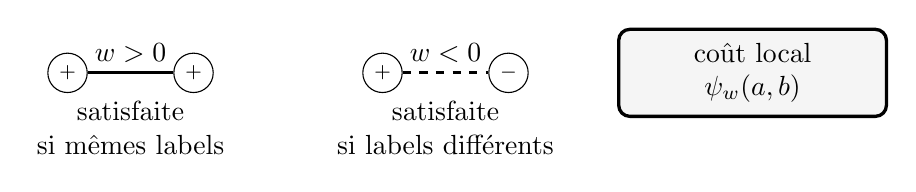
\begin{tikzpicture}[x=1cm,y=1cm]
  \node[spin] (a) at (0,0) {$+$};
  \node[spin] (b) at (1.6,0) {$+$};
  \draw[posedge] (a)--(b) node[midway,above] {$w>0$};
  \node[align=center] at (.8,-.7) {satisfaite\\si mêmes labels};

  \node[spin] (c) at (4,0) {$+$};
  \node[spin] (d) at (5.6,0) {$-$};
  \draw[negedge] (c)--(d) node[midway,above] {$w<0$};
  \node[align=center] at (4.8,-.7) {satisfaite\\si labels différents};

  \node[chapbox,minimum width=3.4cm] at (8.7,0) {coût local\\$\psi_w(a,b)$};
\end{tikzpicture}
\caption{Interprétation d'un poids signé réel. Le signe indique la contrainte préférée ; le module $|w|$ indique la force de cette contrainte.}
\label{fig:chapII_signed_weight}
\end{figure}

\subsection{Frustration}

Dans le cas binaire, une configuration satisfait une arête $e=\{i,j\}$ si
\[
    W_e>0\text{ et }\sigma_i=\sigma_j,
    \qquad\text{ou}\qquad
    W_e<0\text{ et }\sigma_i\neq\sigma_j.
\]

\begin{Definition}{Frustration}{chapII_frustration}
Un graphe signé binaire $(V,E,W)$ est frustré s'il n'existe aucune configuration $\sigma\in\{-1,+1\}^V$ qui satisfasse simultanément toutes les arêtes de poids non nul.
\end{Definition}

\begin{Fait}{Caractérisation de la frustration binaire}{chapII_frustration_parity}
Un graphe signé binaire n'est pas frustré si et seulement si, pour toute paire de sommets $x,y$, la parité du nombre d'arêtes de poids négatif le long d'un chemin reliant $x$ à $y$ ne dépend pas du chemin choisi.
\end{Fait}

\begin{Preuve}
Si une configuration satisfait toutes les arêtes, le produit des signes imposés le long d'un chemin de $x$ à $y$ donne nécessairement le rapport entre les spins en $x$ et en $y$ ; il ne peut donc pas dépendre du chemin. Réciproquement, si cette parité est indépendante du chemin, on fixe un sommet racine et l'on définit le spin d'un sommet par la parité des arêtes négatives le long de n'importe quel chemin depuis la racine. La propriété d'indépendance rend cette définition cohérente et satisfait toutes les arêtes.
\end{Preuve}

\begin{figure}[H]
\centering
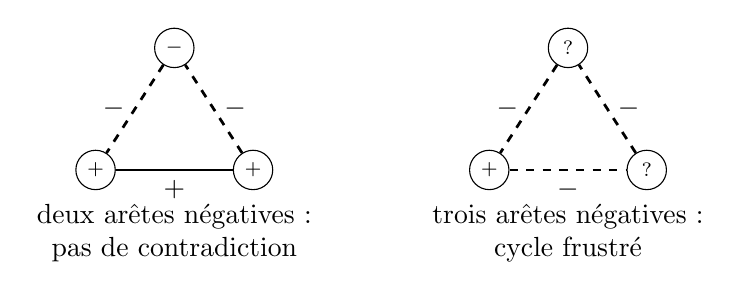
\begin{tikzpicture}[x=1cm,y=1cm]
  \node[spin] (a) at (0,0) {$+$};
  \node[spin] (b) at (2,0) {$+$};
  \node[spin] (c) at (1,1.55) {$-$};
  \draw[posedge] (a)--(b) node[midway,below] {$+$};
  \draw[negedge] (b)--(c) node[midway,right] {$-$};
  \draw[negedge] (c)--(a) node[midway,left] {$-$};
  \node[align=center] at (1,-.8) {deux arêtes négatives :\\pas de contradiction};

  \node[spin] (d) at (5,0) {$+$};
  \node[spin] (e) at (7,0) {$?$};
  \node[spin] (f) at (6,1.55) {$?$};
  \draw[negedge] (d)--(e) node[midway,below] {$-$};
  \draw[negedge] (e)--(f) node[midway,right] {$-$};
  \draw[negedge] (f)--(d) node[midway,left] {$-$};
  \node[align=center] at (6,-.8) {trois arêtes négatives :\\cycle frustré};
\end{tikzpicture}
\caption{La frustration apparaît dès qu'un cycle impose une contradiction. Le triangle pleinement répulsif est le plus petit exemple.}
\label{fig:chapII_frustration_triangle}
\end{figure}

\section{Dynamiques de clusters abstraites}
\label{sec:chapII_cluster_abstrait}

\subsection{Bonds et balance locale}

On suppose que l'énergie est décomposée en contributions locales
\begin{equation}
    U(\sigma)=U_0(\sigma)+\sum_{b\in\mathcal B}U_b(\sigma),
    \label{eq:chapII_bond_decomposition}
\end{equation}
où chaque $b\in\mathcal B$ est un bond : arête, triangle, tétraèdre, ou motif local plus général. Une dynamique de clusters commence par tirer, pour chaque bond $b$, un ensemble de contraintes gelées $\omega_b$ suivant une loi $P_b^\sigma$ dépendant de la configuration courante.

\begin{Definition}{Compatibilité et balance de clusters}{chapII_cluster_balance}
Pour deux configurations $\sigma,\sigma'$ et un bond $b$, on pose
\begin{equation}
    P_b^{\sigma\to\sigma'}(\omega_b)
    =
    \begin{cases}
        P_b^\sigma(\omega_b),&\text{si }P_b^{\sigma'}(\omega_b)>0,\\
        0,&\text{sinon.}
    \end{cases}
    \label{eq:chapII_compatibilite}
\end{equation}
La règle de gel satisfait la balance de clusters si, pour tout $b$, tout $\omega_b$ et toutes configurations $\sigma,\sigma'$,
\begin{equation}
    P_b^{\sigma\to\sigma'}(\omega_b)
    =
    \exp\left[-\left(U_b(\sigma')-U_b(\sigma)\right)\right]
    P_b^{\sigma'\to\sigma}(\omega_b).
    \label{eq:chapII_balance_cluster}
\end{equation}
\end{Definition}

\begin{Theoreme}{Invariance par balance locale}{chapII_invariance_balance}
Supposons que les choix de gel des bonds soient conditionnellement indépendants, que la balance de clusters \eqref{eq:chapII_balance_cluster} soit satisfaite, et que $P_b^\sigma(\varnothing)>0$ pour tout $b$ et tout $\sigma$. Alors la dynamique obtenue après recoloriage des clusters est réversible par rapport à la mesure
\[
    \mu(\sigma)=Z^{-1}e^{-U(\sigma)}.
\]
En particulier, $\mu$ est stationnaire.
\end{Theoreme}

\begin{Preuve}
Soit $T(\sigma,\sigma')$ la probabilité de transition. On somme sur les familles de contraintes gelées compatibles avec $\sigma$ et $\sigma'$. Par indépendance des bonds et par \eqref{eq:chapII_balance_cluster}, chaque famille compatible apporte le facteur
\[
    \prod_{b\in\mathcal B}\exp[-(U_b(\sigma')-U_b(\sigma))]
    =
    \exp[-(U(\sigma')-U(\sigma))].
\]
On obtient
\[
    T(\sigma,\sigma')=\frac{\mu(\sigma')}{\mu(\sigma)}T(\sigma',\sigma),
\]
ce qui est la réversibilité. La condition $P_b^\sigma(\varnothing)>0$ évite de figer irréversiblement une contrainte et donne l'irréductibilité sur le support naturel de la mesure.
\end{Preuve}

\subsection{Le cas arête par arête : \textsc{Swendsen--Wang} signé}

Pour un poids signé réel $W_e$, l'arête est satisfaite si elle respecte la préférence indiquée par le signe de $W_e$. La dynamique arête par arête est alors :
\begin{enumerate}
    \item on ne garde que les arêtes satisfaites par la configuration courante ;
    \item une arête satisfaite $e$ est gelée avec probabilité
    \begin{equation}
        p_e^{\mathrm{gel}}=1-e^{-|W_e|};
        \label{eq:chapII_freeze_edge_weight}
    \end{equation}
    \item chaque cluster gelé est recolorié indépendamment selon la loi conditionnelle prescrite par la mesure cible. Dans le cas binaire sans champ externe, cela revient à retourner ou non le cluster avec probabilité $1/2$.
\end{enumerate}

\begin{Resultat}{Dynamique de \textsc{Swendsen--Wang} signée}{chapII_SW_signed}
La dynamique arête par arête décrite ci-dessus est réversible par rapport à la mesure de \textsc{Gibbs} associée à l'énergie \eqref{eq:chapII_energy_general_weights}--\eqref{eq:chapII_signed_potential}. C'est la dynamique de \SW{} dans le formalisme d'\ES{} \cite{SwendsenWang,EdwardsSokal}.
\end{Resultat}

\begin{figure}[H]
\centering
\begin{tikzpicture}[x=1cm,y=1cm]
  \node at (1.2,2.4) {configuration};
  \foreach \n/\x/\y/\s in {a/0/1/+,b/1.2/1/+,c/2.4/1/-,d/0/0/-,e/1.2/0/-,f/2.4/0/+}
    \node[spin] (\n) at (\x,\y) {$\s$};
  \draw[posedge] (a)--(b);
  \draw[negedge] (b)--(c);
  \draw[posedge] (d)--(e);
  \draw[negedge] (e)--(f);
  \draw[faint] (a)--(d); \draw[faint] (b)--(e); \draw[faint] (c)--(f);

  \draw[chaparr] (3.0,.5)--(4.2,.5);
  \node at (5.8,2.4) {arêtes gelées};
  \foreach \n/\x/\y in {a2/4.8/1,b2/6/1,c2/7.2/1,d2/4.8/0,e2/6/0,f2/7.2/0}
    \node[tinynode] (\n) at (\x,\y) {};
  \draw[freeze] (a2)--(b2); \draw[freeze] (d2)--(e2); \draw[freeze] (c2)--(f2);
  \node[draw,rounded corners,fit=(a2)(b2),inner sep=2pt] {};
  \node[draw,rounded corners,fit=(d2)(e2),inner sep=2pt] {};
  \node[draw,rounded corners,fit=(c2)(f2),inner sep=2pt] {};

  \draw[chaparr] (7.8,.5)--(9.0,.5);
  \node at (10.8,2.4) {recoloriage};
  \foreach \n/\x/\y/\s in {a3/9.6/1/-,b3/10.8/1/-,c3/12/1/+,d3/9.6/0/-,e3/10.8/0/-,f3/12/0/+}
    \node[spin] (\n) at (\x,\y) {$\s$};
  \draw[freeze] (a3)--(b3); \draw[freeze] (d3)--(e3); \draw[freeze] (c3)--(f3);
\end{tikzpicture}
\caption{Un pas de \SW{} signé : on gèle seulement des arêtes satisfaites, puis on recolorie les clusters. La dynamique est correcte pour la mesure cible, mais elle peut geler trop d'information contradictoire dans les systèmes frustrés.}
\label{fig:chapII_SW_step}
\end{figure}

\section{Dynamiques triangulaires et obstruction par percolation}
\label{sec:chapII_triangles_perco}

\subsection{Transfert d'énergie vers les triangles}

Soit $\mathcal T$ une famille de triangles du graphe. Si une arête $e$ appartient à $\mathcal T_e\subseteq\mathcal T$, on peut répartir son poids signé entre les triangles qui la contiennent :
\begin{equation}
    W_{e,t}=\frac{W_e}{|\mathcal T_e|},
    \qquad t\in\mathcal T_e.
    \label{eq:chapII_transfer_weight}
\end{equation}
Les arêtes qui n'appartiennent à aucun triangle restent traitées comme des bonds-arêtes. Comme les coûts locaux sont linéaires en $|W_e|$ à signe fixé, cette opération ne change pas l'énergie totale. Elle change seulement la décomposition en bonds, donc la dynamique de clusters.

\begin{figure}[H]
\centering
\begin{tikzpicture}[x=1cm,y=1cm]
  \node at (1.6,2.8) {bonds-arêtes};
  \foreach \n/\x/\y in {a/0/0,b/1/0,c/2/0,d/.5/.86,e/1.5/.86,f/1/1.72}
    \node[tinynode] (\n) at (\x,\y) {};
  \foreach \u/\v in {a/b,b/c,a/d,b/d,b/e,c/e,d/e,d/f,e/f}
    \draw[posedge] (\u)--(\v);
  \node at (1,-.55) {$W_e$ sur chaque arête};

  \draw[chaparr] (3.1,.8)--(4.5,.8);
  \node[align=center] at (3.8,1.35) {même énergie\\autre décomposition};

  \node at (6.5,2.8) {bonds-triangles};
  \coordinate (a2) at (5,0); \coordinate (b2) at (6,0); \coordinate (c2) at (7,0);
  \coordinate (d2) at (5.5,.86); \coordinate (e2) at (6.5,.86); \coordinate (f2) at (6,1.72);
  \filldraw[triwhite] (a2)--(b2)--(d2)--cycle;
  \filldraw[trigray] (b2)--(d2)--(e2)--cycle;
  \filldraw[triwhite] (b2)--(c2)--(e2)--cycle;
  \filldraw[trigray] (d2)--(e2)--(f2)--cycle;
  \foreach \p in {a2,b2,c2,d2,e2,f2} \node[tinynode] at (\p) {};
  \node at (6,-.55) {$W_{e,t}$ dans les triangles};
\end{tikzpicture}
\caption{Le transfert d'énergie ne change pas la mesure de \textsc{Gibbs}. Il modifie seulement le couplage produit par un pas de dynamique. C'est toute l'astuce, et elle est moins magique qu'elle en a l'air.}
\label{fig:chapII_transfer_energy}
\end{figure}

\subsection{Règles locales sur un triangle isotrope}

Pour $K=2$, les triangles signés se répartissent en deux familles : ceux qui ne portent pas de frustration locale, et ceux qui en portent déjà une. À retournement local de spins près, il suffit d'étudier le triangle pleinement attractif et le triangle pleinement répulsif. Dans le cas isotrope, toutes les arêtes ont même intensité $u>0$. On pose
\begin{equation}
    a_u=1-e^{-2u},
    \qquad
    b_u=e^{-2u}.
    \label{eq:chapII_triangle_ab}
\end{equation}
La dynamique triangulaire gèle moins que la dynamique par arêtes tout en vérifiant la balance locale. Sur un triangle pleinement attractif, l'état de basse énergie $+++$ gèle soit le triangle entier, soit rien ; les autres états ne gèlent rien. Sur un triangle pleinement répulsif, les états de basse énergie gèlent exactement une arête compatible, choisie de façon symétrique.

\begin{figure}[H]
\centering
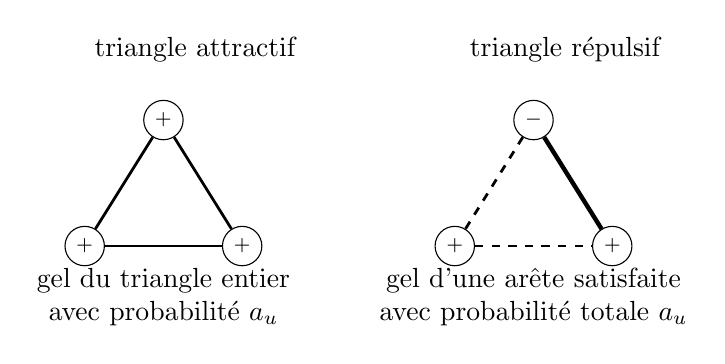
\begin{tikzpicture}[x=1cm,y=1cm]
  \node at (1.4,2.5) {triangle attractif};
  \node[spin] (a) at (0,0) {$+$}; \node[spin] (b) at (2,0) {$+$}; \node[spin] (c) at (1,1.6) {$+$};
  \draw[posedge] (a)--(b); \draw[posedge] (b)--(c); \draw[posedge] (c)--(a);
  \node[align=center] at (1,-.65) {gel du triangle entier\\avec probabilité $a_u$};

  \node at (6.1,2.5) {triangle répulsif};
  \node[spin] (d) at (4.7,0) {$+$}; \node[spin] (e) at (6.7,0) {$+$}; \node[spin] (f) at (5.7,1.6) {$-$};
  \draw[negedge] (d)--(e); \draw[negedge] (e)--(f); \draw[negedge] (f)--(d);
  \draw[freeze] (e)--(f);
  \node[align=center] at (5.7,-.65) {gel d'une arête satisfaite\\avec probabilité totale $a_u$};
\end{tikzpicture}
\caption{Règles locales de la dynamique triangulaire isotrope. Les notations $a_u=1-e^{-2u}$ et $b_u=e^{-2u}$ remplacent les anciennes notations séparées : seule l'intensité $u=|W|$ intervient.}
\label{fig:chapII_triangle_rules}
\end{figure}

\begin{Fait}{Balance locale de la dynamique triangulaire}{chapII_triangle_balance}
Les règles triangulaires isotropes décrites ci-dessus satisfont la balance locale \eqref{eq:chapII_balance_cluster}. Par produit indépendant sur les triangles, la dynamique globale laisse donc invariante la même mesure de \textsc{Gibbs} que la dynamique arête par arête.
\end{Fait}

\begin{Preuve}
Sur un triangle isotrope, il n'y a que deux niveaux d'énergie pertinents dans chacune des deux familles. Les rapports de probabilités de transition entre les états de basse et de haute énergie sont donc imposés par le facteur $e^{-2u}$. Les choix $b_u=e^{-2u}$ et $a_u=1-e^{-2u}$ donnent exactement ces rapports. L'indépendance des bonds permet ensuite de multiplier les identités locales, ce qui donne le Théorème~\ref{th:chapII_invariance_balance}.
\end{Preuve}

\subsection{Percolation nécessaire}

On fixe une suite de modèles et une dynamique de clusters invariante. On note $\kappa_n$ l'objet gelé produit par un pas de dynamique appliqué à une configuration $\Sigma_n\sim\mu_{n,X,W}$, et $\mathcal C(\kappa_n)$ les clusters correspondants.

\begin{Definition}{Masse macroscopique des clusters}{chapII_theta_clusters}
Pour $\delta>0$, on définit
\begin{equation}
    \theta_\delta(\kappa_n)
    =
    \frac1n\sum_{C\in\mathcal C(\kappa_n)}|C|\,\ind{|C|\ge \delta n}.
    \label{eq:chapII_theta_delta}
\end{equation}
On pose ensuite
\begin{equation}
    \theta^{\max}
    =
    \inf\left\{\theta\in[0,1]:
    \lim_{\delta\downarrow0}\limsup_{n\to\infty}
    \mathbb P\left[\theta_\delta(\kappa_n)>\theta\right]=0
    \right\}.
    \label{eq:chapII_theta_max}
\end{equation}
\end{Definition}

La définition ne suppose pas l'unicité d'un cluster géant : $\theta_\delta$ mesure la masse totale portée par tous les clusters de taille au moins $\delta n$.

\begin{Theoreme}{Obstruction générale relative au meilleur random guess}{chapII_general_obstruction_RG}
Supposons que la dynamique de clusters invariante vérifie la propriété suivante : pour tout $\delta>0$ et tout algorithme $\tau_n$,
\begin{equation}
    \mathbb E\left[\ov_n(\Sigma_n^{(1)},\tau_n)\right]
    \le
    \RG_n+
    \mathbb E\left[\theta_\delta(\kappa_n)\right]+r_n(\delta),
    \label{eq:chapII_RG_compatible}
\end{equation}
où
\[
    \lim_{\delta\downarrow0}\limsup_{n\to\infty}r_n(\delta)=0.
\]
Alors tout algorithme satisfait
\begin{equation}
    \limsup_{n\to\infty}
    \left(
    \mathbb E\left[\ov_n(\Sigma_n,\tau_n)\right]-\RG_n
    \right)
    \le
    \theta^{\max}.
    \label{eq:chapII_general_obstruction_RG}
\end{equation}
En particulier, si $\theta^{\max}=0$, le recouvrement partiel au sens de la Définition~\ref{def:chapII_weak_general} est impossible.
\end{Theoreme}

\begin{Preuve}
Par le Corollaire~\ref{cor:chapII_overlap_markov}, on peut remplacer $\Sigma_n$ par $\Sigma_n^{(1)}$ dans l'espérance de recouvrement. L'inégalité \eqref{eq:chapII_RG_compatible} donne ensuite, pour tout $\delta>0$,
\[
    \mathbb E\left[\ov_n(\Sigma_n,\tau_n)\right]-\RG_n
    \le
    \mathbb E\left[\theta_\delta(\kappa_n)\right]+r_n(\delta).
\]
On prend le $\limsup$ en $n$, puis on fait tendre $\delta$ vers $0$. La définition de $\theta^{\max}$ donne le résultat.
\end{Preuve}

\begin{Theoreme}{Version équilibrée : borne explicite}{chapII_balanced_perco_bound}
Supposons $K$ fixé, l'a priori uniforme équilibré, et supposons que les petits clusters soient recoloriés indépendamment et uniformément, comme dans les dynamiques de type \SW{} sans champ externe. Alors
\begin{equation}
    \limsup_{n\to\infty}
    \mathbb E\left[\ov_n(\Sigma_n,\tau_n)\right]
    \le
    \frac1K+\frac{K-1}{K}\theta^{\max}
    \label{eq:chapII_balanced_perco_bound}
\end{equation}
pour toute suite d'algorithmes $\tau_n$. En particulier, si $\theta^{\max}=0$, le recouvrement partiel est impossible.
\end{Theoreme}

\begin{Preuve}
On fixe $\delta>0$. Conditionnellement à la partition gelée, les clusters de taille $<\delta n$ sont recoloriés indépendamment et uniformément. Pour une permutation globale des labels fixée, l'accord moyen sur ces petits clusters a espérance $1/K$ ; sa variance est bornée par une constante fois $\delta$, car chaque bloc pèse au plus $\delta$. Comme $K!$ est fini, le maximum sur les permutations ne change pas le terme d'erreur lorsque $\delta\downarrow0$. Les clusters de taille au moins $\delta n$ peuvent, au pire, être entièrement correctement prédits ; leur contribution est donc majorée par $\theta_\delta(\kappa_n)$. On obtient
\[
    \ov_n(\Sigma_n^{(1)},\tau_n)
    \le
    \frac1K\left(1-\theta_\delta(\kappa_n)\right)
    +\theta_\delta(\kappa_n)
    +o_{\mathbb P}(1)+O(\sqrt{\delta}).
\]
On prend l'espérance, puis les limites $n\to\infty$ et $\delta\downarrow0$, et l'on utilise le Corollaire~\ref{cor:chapII_overlap_markov}.
\end{Preuve}

\begin{figure}[H]
\centering
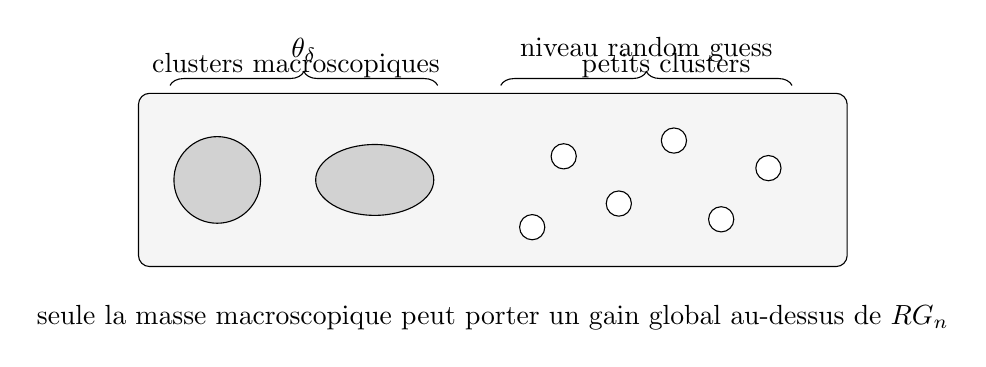
\begin{tikzpicture}[x=1cm,y=1cm]
  \draw[rounded corners,fill=gray!8] (0,0) rectangle (9,2.2);
  \filldraw[fill=gray!35,draw=black] (1.0,1.1) circle (.55);
  \filldraw[fill=gray!35,draw=black] (3.0,1.1) ellipse (.75 and .45);
  \foreach \x/\y in {5/.5,5.4/1.4,6.1/.8,6.8/1.6,7.4/.6,8/1.25}
    \filldraw[fill=white,draw=black] (\x,\y) circle (.16);
  \node at (2,2.55) {clusters macroscopiques};
  \node at (6.7,2.55) {petits clusters};
  \draw[decorate,decoration={brace,amplitude=5pt}] (.4,2.3)--(3.8,2.3) node[midway,above=.18cm] {$\theta_\delta$};
  \draw[decorate,decoration={brace,amplitude=5pt}] (4.6,2.3)--(8.3,2.3) node[midway,above=.18cm] {niveau random guess};
  \node[align=center] at (4.5,-.65) {seule la masse macroscopique peut porter un gain global au-dessus de $\RG_n$};
\end{tikzpicture}
\caption{Principe de la borne de percolation. Les petits clusters sont repeints de façon essentiellement aveugle ; seuls les clusters macroscopiques peuvent transmettre une information globale.}
\label{fig:chapII_perco_obstruction}
\end{figure}

\section*{Sous-partie III --- Applications}
\addcontentsline{toc}{section}{Sous-partie III --- Applications}
\label{sec:chapII_partie_applications}

\section{Le modèle de \textsc{Sankararaman--Baccelli} dans le cadre bayésien}
\label{sec:chapII_SB}

\subsection{Le canal d'observation}

On se donne un graphe potentiel $G=(V,E)$, éventuellement géométrique, et des fonctions de connexion
\[
    f_{\mathrm{in}},f_{\mathrm{out}}:\mathbb R_+\to[0,1],
    \qquad
    f_{\mathrm{in}}(r)\ge f_{\mathrm{out}}(r).
\]
L'a priori sur $\Sigma$ est uniforme dans le modèle original. Conditionnellement à $\Sigma$, une arête potentielle $e=\{i,j\}$, de longueur $r_e=\|x_i-x_j\|$, est observée dans $H$ avec probabilité
\[
    f_{\mathrm{in}}(r_e)\quad\text{si }\Sigma_i=\Sigma_j,
    \qquad
    f_{\mathrm{out}}(r_e)\quad\text{si }\Sigma_i\neq\Sigma_j.
\]

On transforme ensuite l'observation $H$ en poids signés sur toutes les arêtes potentielles :
\begin{equation}
    W_e(H)=
    \begin{cases}
        \displaystyle \log\left(\frac{f_{\mathrm{in}}(r_e)}{f_{\mathrm{out}}(r_e)}\right),& e\in H,\\[2ex]
        \displaystyle -\log\left(\frac{1-f_{\mathrm{out}}(r_e)}{1-f_{\mathrm{in}}(r_e)}\right),& e\notin H.
    \end{cases}
    \label{eq:chapII_SB_weights}
\end{equation}
Les arêtes présentes sont donc attractives ; les arêtes absentes sont répulsives. Les cas limites se traitent avec les conventions usuelles dans $\mathbb R\cup\{\pm\infty\}$.

\begin{Fait}{La postérieure de \textsc{Sankararaman--Baccelli} est une mesure de \textsc{Gibbs} signée}{chapII_SB_posterior}
Dans le modèle de \SB{} avec a priori uniforme, la loi conditionnelle de $\Sigma$ sachant $H$ est exactement la mesure de \textsc{Gibbs}
\begin{equation}
    \mu_H(\sigma)
    =
    \frac1{Z_H}
    \exp\left[-\sum_{e=\{i,j\}\in E}\psi_{W_e(H)}(\sigma_i,\sigma_j)\right],
    \label{eq:chapII_SB_gibbs}
\end{equation}
où $\psi$ est le potentiel signé \eqref{eq:chapII_signed_potential}.
\end{Fait}

\begin{Preuve}
La vraisemblance de $H$ sachant $\sigma$ est
\[
    \prod_{e\in H} f_{\sigma_i,\sigma_j}(r_e)
    \prod_{e\notin H}\left(1-f_{\sigma_i,\sigma_j}(r_e)\right),
\]
où $f_{a,b}=f_{\mathrm{in}}$ si $a=b$ et $f_{a,b}=f_{\mathrm{out}}$ sinon. On factorise les termes ne dépendant pas de $\sigma$. Pour une arête présente, le coût relatif d'une paire de labels différents est
\[
    \log\left(\frac{f_{\mathrm{in}}(r_e)}{f_{\mathrm{out}}(r_e)}\right)=|W_e(H)|.
\]
Pour une arête absente, le coût relatif d'une paire de labels égaux est
\[
    \log\left(\frac{1-f_{\mathrm{out}}(r_e)}{1-f_{\mathrm{in}}(r_e)}\right)=|W_e(H)|.
\]
On obtient donc exactement \eqref{eq:chapII_SB_gibbs}.
\end{Preuve}

\begin{figure}[H]
\centering
\begin{tikzpicture}[x=1cm,y=1cm]
  \node[spin,fill=gray!10] (a) at (0,1) {$+$};
  \node[spin,fill=gray!10] (b) at (1.4,1) {$+$};
  \node[spin,fill=gray!25] (c) at (0,0) {$-$};
  \node[spin,fill=gray!25] (d) at (1.4,0) {$-$};
  \draw[posedge] (a)--(b) node[midway,above] {$H$};
  \draw[posedge] (c)--(d) node[midway,below] {$H$};
  \draw[negedge] (a)--(c) node[midway,left] {$E\setminus H$};
  \draw[negedge] (b)--(d) node[midway,right] {$E\setminus H$};
  \node[align=center] at (.7,-.9) {présence $\Rightarrow W_e>0$\\absence $\Rightarrow W_e<0$};

  \draw[chaparr] (2.5,.5)--(3.7,.5);
  \node[chapbox,minimum width=4cm] at (5.8,.5) {postérieure\\$\mu_H(\sigma)\propto e^{-U_H(\sigma)}$\\avec poids $W_e(H)$};
\end{tikzpicture}
\caption{Dans le modèle de \SB{}, l'observation d'un sous-graphe $H$ se traduit naturellement en graphe signé pondéré. Il n'y a pas besoin de deux familles de paramètres : un seul poids signé $W_e(H)$ suffit.}
\label{fig:chapII_SB_weights}
\end{figure}

\section{Retrouver la borne de \textsc{Sankararaman--Baccelli} par \textsc{Swendsen--Wang} arêtes}
\label{sec:chapII_SB_edges}

Appliquons un pas de \SW{} arête par arête à une configuration postérieure. Sous le modèle génératif de \SB{}, conditionnellement à la vérité $\Sigma$, examinons une arête potentielle $e=\{i,j\}$ de longueur $r_e$.

Si $\Sigma_i=\Sigma_j$, l'arête est présente avec probabilité $f_{\mathrm{in}}(r_e)$. Lorsqu'elle est présente, son poids est positif et vaut en module
\[
    \log\left(\frac{f_{\mathrm{in}}(r_e)}{f_{\mathrm{out}}(r_e)}\right).
\]
Elle est donc gelée avec probabilité
\[
    1-\frac{f_{\mathrm{out}}(r_e)}{f_{\mathrm{in}}(r_e)}.
\]
La probabilité totale de gel est
\begin{equation}
    f_{\mathrm{in}}(r_e)
    \left(1-\frac{f_{\mathrm{out}}(r_e)}{f_{\mathrm{in}}(r_e)}\right)
    =
    f_{\mathrm{in}}(r_e)-f_{\mathrm{out}}(r_e).
    \label{eq:chapII_SB_edge_same}
\end{equation}

Si $\Sigma_i\neq\Sigma_j$, l'arête absente est satisfaite comme interaction répulsive. Elle est absente avec probabilité $1-f_{\mathrm{out}}(r_e)$, et son poids négatif a pour module
\[
    \log\left(\frac{1-f_{\mathrm{out}}(r_e)}{1-f_{\mathrm{in}}(r_e)}\right).
\]
La probabilité totale de gel vaut encore
\begin{equation}
    \left(1-f_{\mathrm{out}}(r_e)\right)
    \left(1-\frac{1-f_{\mathrm{in}}(r_e)}{1-f_{\mathrm{out}}(r_e)}\right)
    =
    f_{\mathrm{in}}(r_e)-f_{\mathrm{out}}(r_e).
    \label{eq:chapII_SB_edge_diff}
\end{equation}

\begin{Corollaire}{Réduction à la percolation $f_{\mathrm{in}}-f_{\mathrm{out}}$}{chapII_SB_perco_edges}
Dans le modèle de \SB{}, le graphe gelé produit par un pas de \SW{} arête par arête a même loi qu'une percolation indépendante sur le graphe potentiel, où l'arête $e$ est conservée avec probabilité
\begin{equation}
    f_{\mathrm{in}}(r_e)-f_{\mathrm{out}}(r_e).
    \label{eq:chapII_fin_fout}
\end{equation}
Si cette percolation ne possède pas de composante géante, le recouvrement partiel est impossible.
\end{Corollaire}

Ce corollaire redonne la borne de \SB{} : le couplage par \SW{} arête par arête convertit le problème de récupération en une question de percolation du graphe de paramètre $f_{\mathrm{in}}-f_{\mathrm{out}}$.

\section{La grille triangulaire : une borne strictement meilleure}
\label{sec:chapII_triangular_grid}

\subsection{Modèle homogène sur la grille triangulaire}

On considère maintenant le cas homogène sur la grille triangulaire :
\[
    f_{\mathrm{in}}\equiv p,
    \qquad
    f_{\mathrm{out}}\equiv 1-p,
    \qquad
    p\in\left[\frac12,1\right).
\]
Tous les poids non nuls ont alors le même module
\begin{equation}
    u_p=\log\left(\frac{p}{1-p}\right).
    \label{eq:chapII_up}
\end{equation}
Le signe du poids dépend seulement de la présence ou de l'absence de l'arête observée.

\subsection{Dynamique par arêtes}

Une arête en accord avec la vérité apparaît comme une interaction satisfaite avec probabilité $p$. Conditionnellement à cela, la probabilité de gel vaut
\[
    1-e^{-u_p}=1-\frac{1-p}{p}=\frac{2p-1}{p}.
\]
Donc la probabilité effective de conservation d'une arête dans le graphe gelé est
\begin{equation}
    p_{\mathrm{bond}}=2p-1.
    \label{eq:chapII_pbond_edges}
\end{equation}
Le seuil critique de percolation par arêtes de la grille triangulaire vaut $2\sin(\pi/18)$ ; dans le paramètre $p$, cela donne
\begin{equation}
    p_c^{\mathrm{edge}}
    =
    \frac12+\sin\left(\frac\pi{18}\right)
    =0.673\ldots
    \label{eq:chapII_pc_edges}
\end{equation}
Ainsi, la borne obtenue par \SW{} arête par arête interdit le recouvrement partiel pour
\[
    p<p_c^{\mathrm{edge}}.
\]
Au-delà, cette dynamique ne permet plus de conclure.

\subsection{Dynamique triangulaire}

Sur la grille triangulaire, on choisit une famille de triangles blancs de sorte que chaque arête appartienne à un unique triangle blanc, à effet de bord négligeable. Chaque poids d'arête est transféré à ce triangle. La dynamique de clusters utilise donc des bonds triangulaires corrélés.

Le résultat de percolation corrélée pertinent donne le seuil
\begin{equation}
    p_c^{\triangle}
    =
    \frac74-\frac{\sqrt{17}}4
    =0.7192\ldots
    \label{eq:chapII_pc_triangles}
\end{equation}
\cite{PercolationGrilleTrianglesCorrelations}. Comme
\begin{equation}
    p_c^{\mathrm{edge}}<p_c^{\triangle},
    \label{eq:chapII_pc_comparison}
\end{equation}
la dynamique triangulaire donne une zone supplémentaire de non-recouvrement partiel.

\begin{Corollaire}{Amélioration stricte de la borne sur la grille triangulaire}{chapII_triangle_improvement}
Dans le modèle homogène de \SB{} sur la grille triangulaire, pour tout
\begin{equation}
    p\in
    \left[
    \frac12+\sin\left(\frac\pi{18}\right),
    \frac74-\frac{\sqrt{17}}4
    \right),
    \label{eq:chapII_interval_improvement}
\end{equation}
la dynamique \SW{} arête par arête ne fournit plus d'obstruction, tandis que la dynamique triangulaire ne percole toujours pas. Le recouvrement partiel est donc impossible dans tout cet intervalle.
\end{Corollaire}

\begin{Preuve}
La première borne est obtenue par la percolation indépendante d'arêtes de paramètre $2p-1$, donc par \eqref{eq:chapII_pc_edges}. La dynamique triangulaire, elle, produit le modèle de percolation corrélée dont le seuil est \eqref{eq:chapII_pc_triangles}. Dans l'intervalle \eqref{eq:chapII_interval_improvement}, les clusters triangulaires restent sous-critiques. Le Théorème~\ref{th:chapII_balanced_perco_bound} interdit alors le recouvrement partiel. La stricte amélioration vient de \eqref{eq:chapII_pc_comparison}.
\end{Preuve}

\begin{figure}[H]
\centering
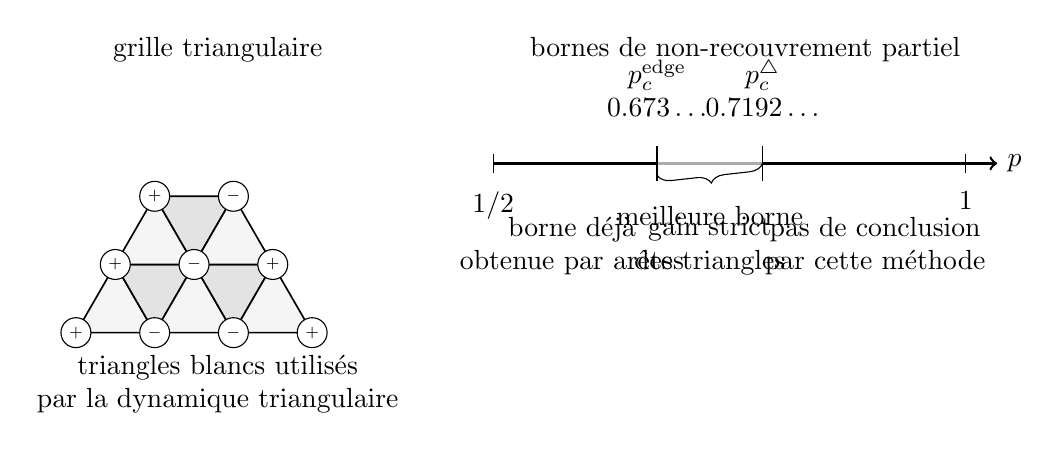
\begin{tikzpicture}[x=1cm,y=1cm]
  % triangular grid left
  \begin{scope}[shift={(0,0)}]
    \node at (1.8,3.6) {grille triangulaire};
    \coordinate (a) at (0,0); \coordinate (b) at (1,0); \coordinate (c) at (2,0); \coordinate (d) at (3,0);
    \coordinate (e) at (.5,.866); \coordinate (f) at (1.5,.866); \coordinate (g) at (2.5,.866);
    \coordinate (h) at (1,1.732); \coordinate (i) at (2,1.732);
    \filldraw[triwhite] (a)--(b)--(e)--cycle;
    \filldraw[trigray] (b)--(e)--(f)--cycle;
    \filldraw[triwhite] (b)--(c)--(f)--cycle;
    \filldraw[trigray] (c)--(f)--(g)--cycle;
    \filldraw[triwhite] (c)--(d)--(g)--cycle;
    \filldraw[triwhite] (e)--(f)--(h)--cycle;
    \filldraw[trigray] (f)--(h)--(i)--cycle;
    \filldraw[triwhite] (f)--(g)--(i)--cycle;
    \foreach \p/\s in {a/+,b/-,c/-,d/+,e/+,f/-,g/+,h/+,i/-}
      \node[tinynode] at (\p) {$\s$};
    \node[align=center] at (1.8,-.65) {triangles blancs utilisés\\par la dynamique triangulaire};
  \end{scope}

  % number line right
  \begin{scope}[shift={(5.3,.55)}]
    \node at (3.2,3.05) {bornes de non-recouvrement partiel};
    \draw[->,line width=.9pt] (0,1.6)--(6.4,1.6) node[right] {$p$};
    \draw (0,1.48)--(0,1.72) node[below=.35cm] {$1/2$};
    \draw (6,1.48)--(6,1.72) node[below=.35cm] {$1$};
    \coordinate (pe) at (2.08,1.6);
    \coordinate (pt) at (3.42,1.6);
    \draw[very thick] (0,1.6)--(pe);
    \draw[very thick,gray!65] (pe)--(pt);
    \draw[dashed] (pt)--(6,1.6);
    \draw (pe)+(0,-.22)--+(0,.22) node[above=.25cm,align=center] {$p_c^{\mathrm{edge}}$\\$0.673\ldots$};
    \draw (pt)+(0,-.22)--+(0,.22) node[above=.25cm,align=center] {$p_c^{\triangle}$\\$0.7192\ldots$};
    \node[align=center] at (1.0,.55) {borne déjà\\obtenue par arêtes};
    \node[align=center] at (2.75,.55) {gain strict\\des triangles};
    \node[align=center] at (4.85,.55) {pas de conclusion\\par cette méthode};
    \draw[decorate,decoration={brace,mirror,amplitude=5pt}] (pe)+(0,-.15)--(pt)+(0,-.15) node[midway,below=.35cm] {meilleure borne};
  \end{scope}
\end{tikzpicture}
\caption{À gauche : choix d'une famille de triangles blancs sur la grille triangulaire. À droite : comparaison des seuils. La dynamique triangulaire étend strictement la zone où l'on prouve l'impossibilité du recouvrement partiel.}
\label{fig:chapII_triangular_bounds}
\end{figure}

\begin{figure}[H]
\centering
\begin{tikzpicture}[x=1cm,y=1cm]
  \node[chapboxdark,minimum width=3.2cm] (obs) at (0,0) {observation\\$H$};
  \node[chapbox,minimum width=3.2cm] (weights) at (4,0) {poids signés\\$W_e(H)$};
  \node[chapbox,minimum width=3.2cm] (mcmc) at (8,0) {dynamique\\triangulaire};
  \node[chapbox,minimum width=3.2cm] (corr) at (4,-1.8) {corrélations\\$\widehat{\mathbb P}(\sigma_i=\sigma_j)$};
  \node[chapbox,minimum width=3.2cm] (cluster) at (8,-1.8) {clustering final\\spectral, \textsc{Leiden}, etc.};
  \draw[chaparr] (obs)--(weights);
  \draw[chaparr] (weights)--(mcmc);
  \draw[chaparr] (mcmc)--(corr);
  \draw[chaparr] (corr)--(cluster);
\end{tikzpicture}
\caption{Pipeline algorithmique suggéré : transformer l'observation en poids signés, échantillonner la postérieure par une dynamique de clusters, estimer les corrélations, puis appliquer un algorithme de clustering standard sur la matrice obtenue.}
\label{fig:chapII_pipeline_algo}
\end{figure}

\section{Ouverture : dimension un et assemblage d'haplotypes}
\label{sec:chapII_haplotypes}

Le même cadre peut être relu en dimension un. Dans l'assemblage d'haplotypes, les sommets correspondent à des positions génomiques ou à des fragments, et les observations donnent des contraintes locales bruitées indiquant si deux éléments proviennent du même haplotype ou de deux haplotypes différents. On obtient donc naturellement un graphe signé pondéré, souvent très local, avec deux communautés cachées. Le travail de \textsc{Sankararaman}, \textsc{Vikalo} et \textsc{Baccelli} \cite{SankararamanVikaloBaccelli2020} s'inscrit dans cette direction.

Dans ce cas, la géométrie unidimensionnelle change la nature de la percolation, mais pas la logique bayésienne : définir la postérieure, comparer l'algorithme au meilleur random guess, puis chercher une dynamique invariante dont les clusters portent l'information pertinente. Encore une fois, le problème n'est pas seulement de produire une partition ; c'est de comprendre quelle information globale subsiste dans la loi postérieure.

\section{Conclusion}
\label{sec:chapII_conclusion}

Le chapitre a construit un cadre bayésien général pour la détection de communautés sur graphes pondérés. Dans ce cadre :
\begin{enumerate}
    \item un algorithme est un noyau fondé sur l'observation ;
    \item un random guess est un noyau qui ne voit pas la réalisation observée ;
    \item le recouvrement partiel signifie battre asymptotiquement le meilleur random guess ;
    \item la vérité cachée peut être remplacée en moyenne par une réplique postérieure ;
    \item toute dynamique de \textsc{Markov} invariante fournit donc un couplage utile ;
    \item les dynamiques de clusters donnent des obstructions par percolation.
\end{enumerate}

Le modèle de \SB{} apparaît alors comme un cas particulier où les poids signés sont explicitement obtenus à partir de l'observation. La dynamique \SW{} arête par arête redonne la borne classique en $f_{\mathrm{in}}-f_{\mathrm{out}}$. Sur la grille triangulaire, le passage à des bonds triangulaires donne une borne strictement meilleure. Le cadre est donc à la fois plus général que le modèle initial et suffisamment concret pour produire immédiatement des résultats théoriques vérifiables.
